
\documentclass{standalone}
\usepackage{xcolor}
\usepackage{pgfplots}
\pgfplotsset{compat=1.18}

\begin{document}

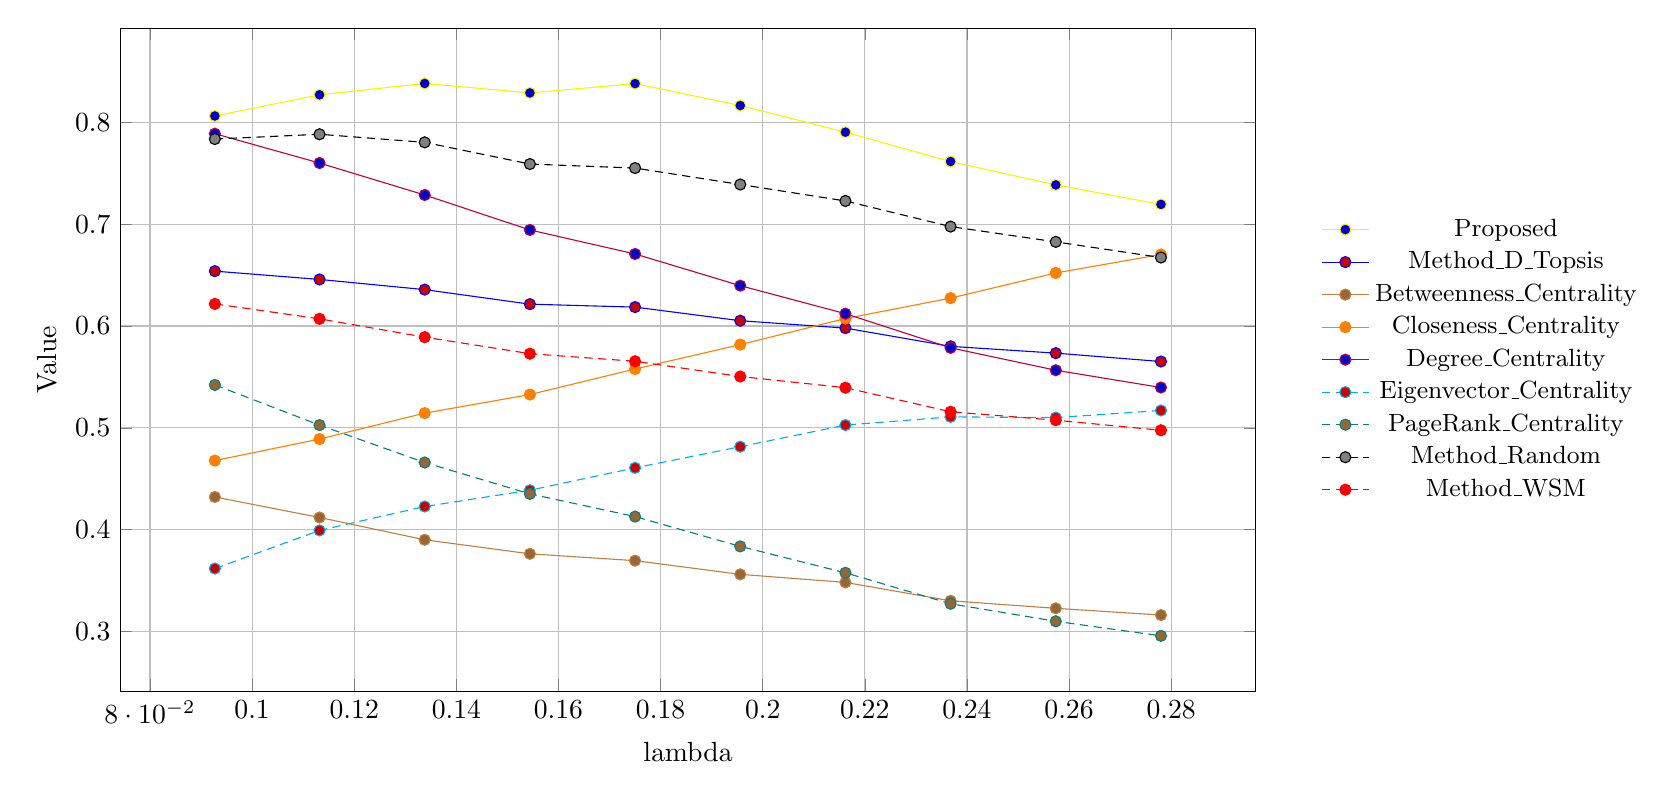
\begin{tikzpicture}
\begin{axis}[
    width=16cm,
    height=10cm,
    xlabel={lambda},
    ylabel={Value},
    grid=major,
    legend style={
        at={(1.05,0.5)},
        anchor=west,
        font=\small,
        draw=none,
        cells={align=left},
    },
]
% Proposed
\addplot+[color=yellow, mark=*] coordinates {
(0.0927,0.8061542723974015) (0.1132,0.826947399561264) (0.1338,0.8380709449929284) (0.1544,0.8287963186869618) (0.175,0.837962942271326) (0.1956,0.8164096092339959) (0.2162,0.7902532764441671) (0.2368,0.7614315923246271) (0.2574,0.7384714482923629) (0.278,0.7193560893474269) };
\addlegendentry{Proposed}

% Method\_D\_Topsis
\addplot+[color=blue, mark=*] coordinates {
(0.0927,0.6538340560068467) (0.1132,0.6456979258816559) (0.1338,0.6357034459441269) (0.1544,0.6214121285737427) (0.175,0.618531041952532) (0.1956,0.6051838927867834) (0.2162,0.5979192853568975) (0.2368,0.5800109323195409) (0.2574,0.5733335539090325) (0.278,0.5651199392798528) };
\addlegendentry{Method\_D\_Topsis}

% Betweenness\_Centrality
\addplot+[color=brown, mark=*] coordinates {
(0.0927,0.4321621449685263) (0.1132,0.4120162291998913) (0.1338,0.3901097670894934) (0.1544,0.3763573022959756) (0.175,0.3696374216186548) (0.1956,0.3561973733021847) (0.2162,0.348284228682427) (0.2368,0.3302379306244892) (0.2574,0.3228419502595248) (0.278,0.3162333096607451) };
\addlegendentry{Betweenness\_Centrality}

% Closeness\_Centrality
\addplot+[color=orange, mark=*] coordinates {
(0.0927,0.4678491588003231) (0.1132,0.4890185131342972) (0.1338,0.5144470729658535) (0.1544,0.5326936450949273) (0.175,0.5577791075322479) (0.1956,0.5817296841774334) (0.2162,0.607312385975698) (0.2368,0.627344185687579) (0.2574,0.652067222679197) (0.278,0.6701914414722964) };
\addlegendentry{Closeness\_Centrality}

% Degree\_Centrality
\addplot+[color=purple, mark=*] coordinates {
(0.0927,0.7887389815290152) (0.1132,0.7599459638014622) (0.1338,0.7285828080631064) (0.1544,0.6942819643642159) (0.175,0.6706871259201048) (0.1956,0.6395838372227095) (0.2162,0.6120781174309051) (0.2368,0.5785396333758721) (0.2574,0.5565583643394914) (0.278,0.5395976255139782) };
\addlegendentry{Degree\_Centrality}

% Eigenvector\_Centrality
\addplot+[color=cyan, mark=*] coordinates {
(0.0927,0.3618999190888312) (0.1132,0.3993198424558231) (0.1338,0.422778385730766) (0.1544,0.4387596235153612) (0.175,0.4607473221210927) (0.1956,0.4814897350578195) (0.2162,0.502731605923739) (0.2368,0.5107931887865469) (0.2574,0.5100628475520558) (0.278,0.5170766699187043) };
\addlegendentry{Eigenvector\_Centrality}

% PageRank\_Centrality
\addplot+[color=teal, mark=*] coordinates {
(0.0927,0.5421123815038654) (0.1132,0.5027050590653237) (0.1338,0.4659862924037051) (0.1544,0.4351754979506622) (0.175,0.4128867125222569) (0.1956,0.3836270973071159) (0.2162,0.3577022680998026) (0.2368,0.3273163063164719) (0.2574,0.3101105670346528) (0.278,0.2958232655755967) };
\addlegendentry{PageRank\_Centrality}

% Method\_Random
\addplot+[color=black, mark=*] coordinates {
(0.0927,0.7835130441340786) (0.1132,0.7882068153916395) (0.1338,0.7802587763135609) (0.1544,0.7589659166464082) (0.175,0.7550271054739045) (0.1956,0.7388811707078679) (0.2162,0.7227262137331945) (0.2368,0.6975656218564242) (0.2574,0.6825660161164593) (0.278,0.6671937373399304) };
\addlegendentry{Method\_Random}

% Method\_WSM
\addplot+[color=red, mark=*] coordinates {
(0.0927,0.6216619184994144) (0.1132,0.6070243746922273) (0.1338,0.5890401687050079) (0.1544,0.5728025851302806) (0.175,0.565362137731729) (0.1956,0.5504103627350876) (0.2162,0.5394098995180379) (0.2368,0.515793514819283) (0.2574,0.5075395754166567) (0.278,0.4976159248408223) };
\addlegendentry{Method\_WSM}


\end{axis}
\end{tikzpicture}

\end{document}
